% Provide your results:
%       clearly

The primary outcome of this work is a mulitdimensional database of repository temperature 
change per mass of high heat contributing isotopes supporting the implementation 
of the \gls{STC} method in \Cyder. 

A validation effort concerning this tool was performed to assess the validity of 
the \gls{STC} method for the purpose of repository thermal response estimation.  
Comparison of the results of this method with the \gls{LLNL} model 
\cite{greenberg_application_2012} gave 
appropriately accurate results and demonstrated the way in which inaccuracies 
from neglected low heat contributing nuclides are bounded. Figure 
\ref{fig:CmValidation} shows the results of one example validation exercise 
comparing the combined scaling and  superposition calculations demonstrated in 
Figures \ref{fig:CmScaling} and \ref{fig:CmSuperposition} respectively. This 
particular validation example, containing no neglected nuclides, demonstrates 
an average error of 1.1\% and a maximum error of 4.4\%.

\begin{figure}[htp!]
\begin{center}
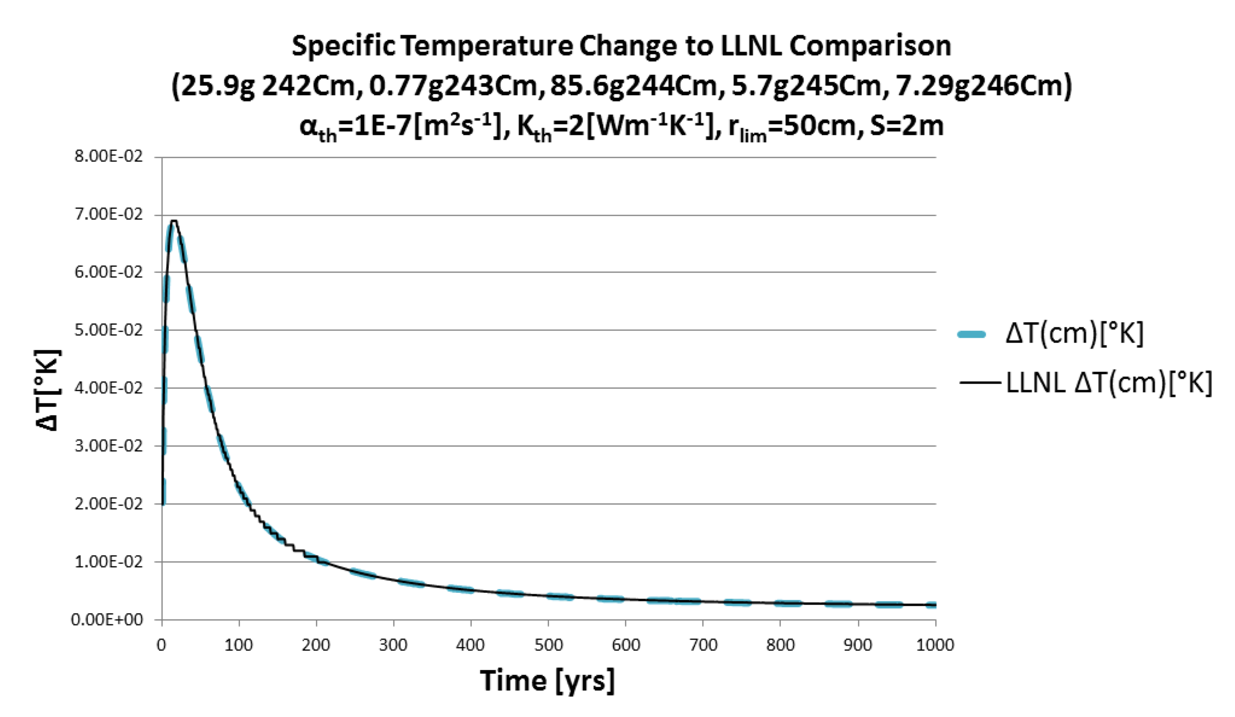
\includegraphics[width=\columnwidth]{./chapters/methodology/thermal_models/CmValidation.eps}
\end{center}
\caption{This comparison of \gls{STC} calculated thermal response from $Cm$ 
inventory per MTHM in 51GWd burnup UOX PWR fuel compares favorably with results 
from the analytical model from LLNL.} 
\label{fig:CmValidation}
\end{figure}

% Unit Test Results
In addition to this validation effort, continual verification of code behavior
is enabled by a suite of unit tests packaged with the tool. These tests may
continually be performed to evaluate the implementated behavior of units of
functionality within the interpolation and specific temperature change
algorithms even as the code is improved in the future.  
